\chapter{Appendix}
\label{app:appendixa}


\section{CPS Statistics}
\label{app:cps}

\subsection{Main Robocup Dataset Environment}
\label{app:mrd}

\begin{figure}[ht!]
\begin{minipage}[b]{0.5\linewidth}
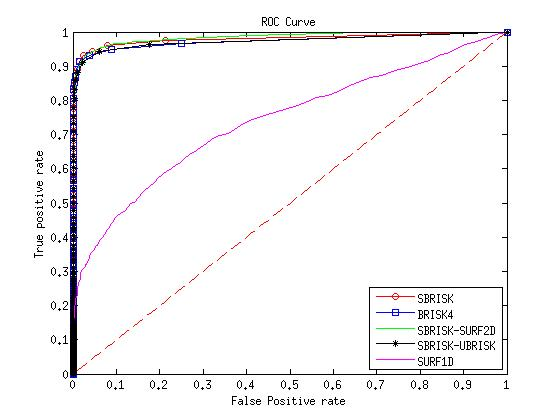
\includegraphics[scale=0.4]{../Drawings/RobocupDataset/ROC_General_KNN_consistent.jpg}
\caption{A comparison of the ROC curves for the Robocup datasets using 2-NN for matching and CPS values}
\label{fig:compareKNNConsist}
\end{minipage}
\hspace{0.5cm}
\begin{minipage}[b]{0.5\linewidth}
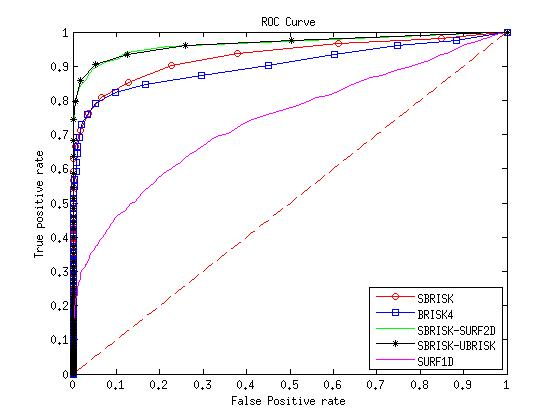
\includegraphics[scale=0.4]{../Drawings/RobocupDataset/ROC_General_Hamming_consistent.jpg}
\caption{A comparison of the ROC curves for the Robocup datasets using Radius Matching and CPS values}
\label{fig:compareHammingConsistent}
\end{minipage}
\end{figure}


\begin{table}


\caption{The AUC and performance statistics for the Main Robocup Dataset using
2-NN using CPS parameters}


\begin{tabular}{|c|c|c|c|c|c|c|c|}
\hline 
\textbf{Method (2-NN)} & \textbf{Parameters} & \textbf{\% AUC} & \textbf{Detection} & \textbf{Extraction} & \textbf{Matching} & \textbf{Verification} & \textbf{Overall}\tabularnewline
 &  &  & \textbf{Time (ms)} & \textbf{Time (ms)} & \textbf{Time (ms)} & \textbf{Time (ms)} & \textbf{Time (ms)}\tabularnewline
\hline 
\hline 
BRISK0 & CPS & 98.000 & 3.863 & 8.342 & 3.380 & 0.039 & 19.622\tabularnewline
\hline 
BRISK4 & CPS & 97.388 & 14.214 & 8.912 & 4.057 & 0.045 & 31.304\tabularnewline
\hline 
BRISK0-SURF2D & CPS & 98.498 & 3.872 & 15.580 & 0.852 & 0.048 & 24.358\tabularnewline
\hline 
BRISK0-UBRISK & CPS & 97.375 & 3.619 & 3.285 & 2.020 & 0.032 & 12.934\tabularnewline
\hline 
\end{tabular}
\label{app:mrd_knn}
\end{table}



\begin{table}
\caption{The AUC and performance statistics for the Main Robocup Dataset using
Radius Matching using CPS parameters}


\begin{tabular}{|c|c|c|c|c|c|c|c|}
\hline 
\textbf{Method (2-NN)} & \textbf{Parameters} & \textbf{\% AUC} & \textbf{Detection} & \textbf{Extraction} & \textbf{Matching} & \textbf{Verification} & \textbf{Overall}\tabularnewline
 &  &  & \textbf{Time (ms)} & \textbf{Time (ms)} & \textbf{Time (ms)} & \textbf{Time (ms)} & \textbf{Time (ms)}\tabularnewline
\hline 
\hline 
BRISK0 & CPS & 92.952 & 2.980 & 2.666 & 0.227 & 0.015 & 9.818\tabularnewline
\hline 
BRISK4 & CPS & 90.343 & 8.577 & 3.229 & 0.355 & 0.027 & 16.173\tabularnewline
\hline 
BRISK0-SURF2D & CPS & 96.503 & 3.181 & 6.406 & 0.218 & 0.008 & 13.815\tabularnewline
\hline 
BRISK0-UBRISK & CPS & 96.637 & 2.943 & 1.675 & 0.215 & 0.010 & 8.755\tabularnewline
\hline 
\end{tabular}
\label{app:mrd_hamming}
\end{table}

\begin{table}
\caption{The number of Image Zero Matches (IZMs) for each feature extraction
algorithm using 2-NN and Radius Matching in the Main Robocup Environment}
\begin{tabular}{|c|c|}
\hline 
\textbf{Method} & \multicolumn{1}{c|}{\textbf{Image Zero Matches}}\tabularnewline
\hline 
 & \multicolumn{1}{c|}{\textbf{2-NN Matching}}\tabularnewline
\hline 
 & \textbf{CPS}\tabularnewline
\hline 
\hline 
BRISK0 & 35.00\tabularnewline
\hline 
BRISK & 63.00\tabularnewline
\hline 
BRISK0- SURF2D & 5.00\tabularnewline
\hline 
UBRISK & 156.00\tabularnewline
\hline 
1D SURF & 17.00\tabularnewline
\hline 
 & \multicolumn{1}{c|}{\textbf{Radius Matching}}\tabularnewline
\hline 
BRISK0 & 21.00\tabularnewline
\hline 
BRISK & 24.00\tabularnewline
\hline 
BRISK0- SURF2D & 57.00\tabularnewline
\hline 
UBRISK & 29.00\tabularnewline
\hline 
1D SURF & 17.00\tabularnewline
\hline 
\end{tabular}
\label{app:mrd_izm}
\end{table}

\begin{figure}
  \centering
    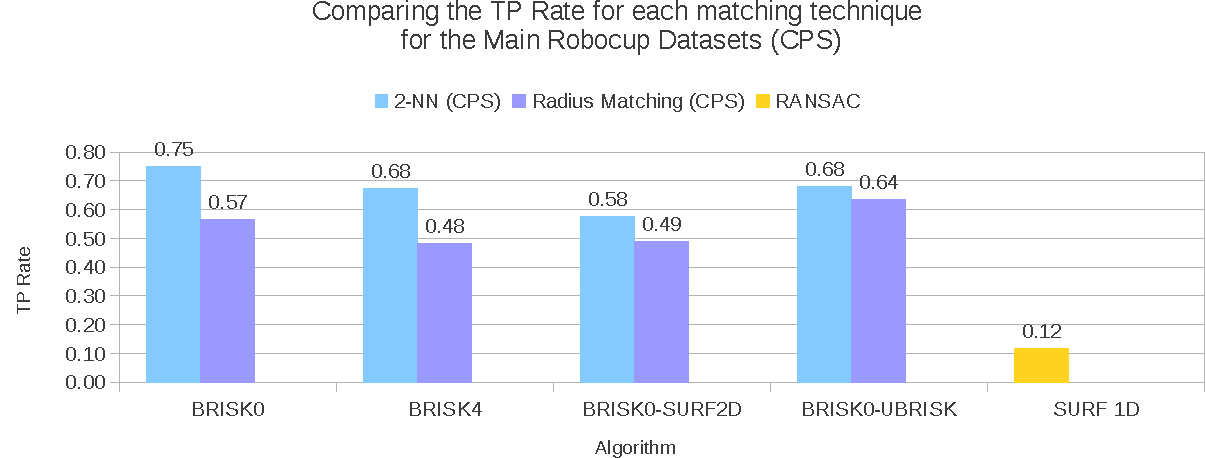
\includegraphics[width=1.0\textwidth]{../Drawings/Graphs/tp_rate_mrb_cps.pdf}
    \caption{The $TP_{FP=0}^{max}$ rate for the Main Robocup datasets} 
    \label{app:tp_rate_mrd}
\end{figure}



\subsection{Office Environment}
\label{app:oe}

\begin{figure}[ht!]
\begin{minipage}[b]{0.5\linewidth}
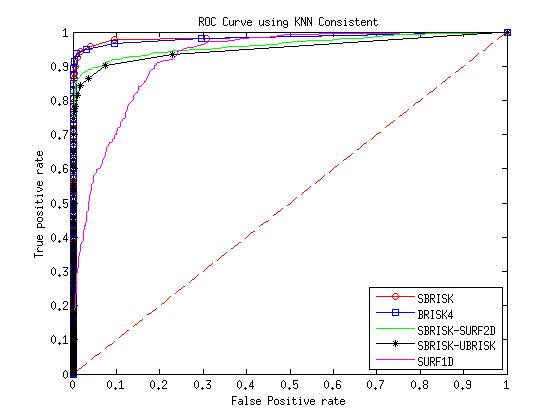
\includegraphics[scale=0.4]{../Drawings/dataset2_ROC_General_KNN_Consistent.jpg}
\caption{A comparison of the ROC curves in the office environment using the CPS thresholds}
\label{fig:compareKnnConsistentOffice}
\end{minipage}
\hspace{0.5cm}
\begin{minipage}[b]{0.5\linewidth}
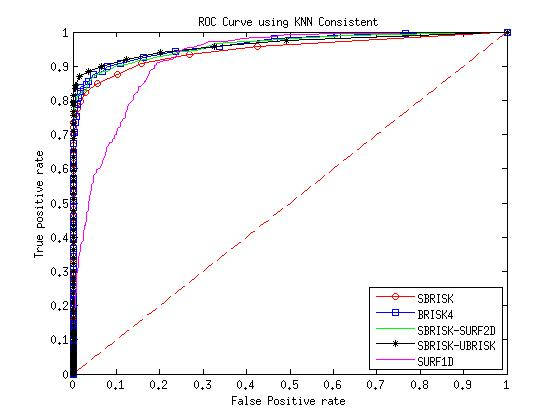
\includegraphics[scale=0.4]{../Drawings/dataset2_ROC_General_Hamming_Consistent.jpg}
\caption{A comparison of the ROC curves in the office environment using the CPS Hamming/Euclidean distance thresholds}
\label{fig:compareHammingConsistentOffice}
\end{minipage}
\end{figure}

\begin{table}
\caption{The AUC and performance statistics for the Office Environment Datasets
using 2-NN using CPS parameters}
\begin{tabular}{|c|c|c|c|c|c|c|c|}
\hline 
\textbf{Method (2-NN)} & \textbf{Parameters} & \textbf{\% AUC} & \textbf{Detection} & \textbf{Extraction} & \textbf{Matching} & \textbf{Verification} & \textbf{Overall}\tabularnewline
 &  &  & \textbf{Time (ms)} & \textbf{Time (ms)} & \textbf{Time (ms)} & \textbf{Time (ms)} & \textbf{Time (ms)}\tabularnewline
\hline 
\hline 
BRISK0 & CPS & 98.457 & 4.499 & 14.911 & 17.984 & 0.112 & 41.889\tabularnewline
\hline 
BRISK4 & CPS & 98.282 & 18.546 & 15.856 & 24.097 & 0.137 & 63.065\tabularnewline
\hline 
BRISK0-SURF2D & CPS & 96.210 & 4.520 & 28.129 & 3.600 & 0.131 & 40.822\tabularnewline
\hline 
BRISK0-UBRISK & CPS & 95.182 & 4.149 & 5.298 & 11.723 & 0.090 & 25.666\tabularnewline
\hline 
\end{tabular}
\label{app:oe_knn}
\end{table}

\begin{table}
\caption{The AUC and performance statistics for the Office Environment Datasets
using Radius Macthing and CPS parameters}
\begin{tabular}{|c|c|c|c|c|c|c|c|}
\hline 
\textbf{Method (2-NN)} & \textbf{Parameters} & \textbf{\% AUC} & \textbf{Detection} & \textbf{Extraction} & \textbf{Matching} & \textbf{Verification} & \textbf{Overall}\tabularnewline
 &  &  & \textbf{Time (ms)} & \textbf{Time (ms)} & \textbf{Time (ms)} & \textbf{Time (ms)} & \textbf{Time (ms)}\tabularnewline
\hline 
\hline 
BRISK0 & CPS & 94.697 & 3.118 & 3.590 & 0.889 & 0.014 & 11.948\tabularnewline
\hline 
BRISK4 & CPS & 96.274 & 9.997 & 4.663 & 2.082 & 0.023 & 21.164\tabularnewline
\hline 
BRISK0-SURF2D & CPS & 96.084 & 3.366 & 10.196 & 0.656 & 0.022 & 18.577\tabularnewline
\hline 
BRISK0-UBRISK & CPS & 96.277 & 3.120 & 2.060 & 0.875 & 0.017 & 10.409\tabularnewline
\hline 
\end{tabular}
\label{app:oe_hamming}
\end{table}

\begin{figure}
  \centering
    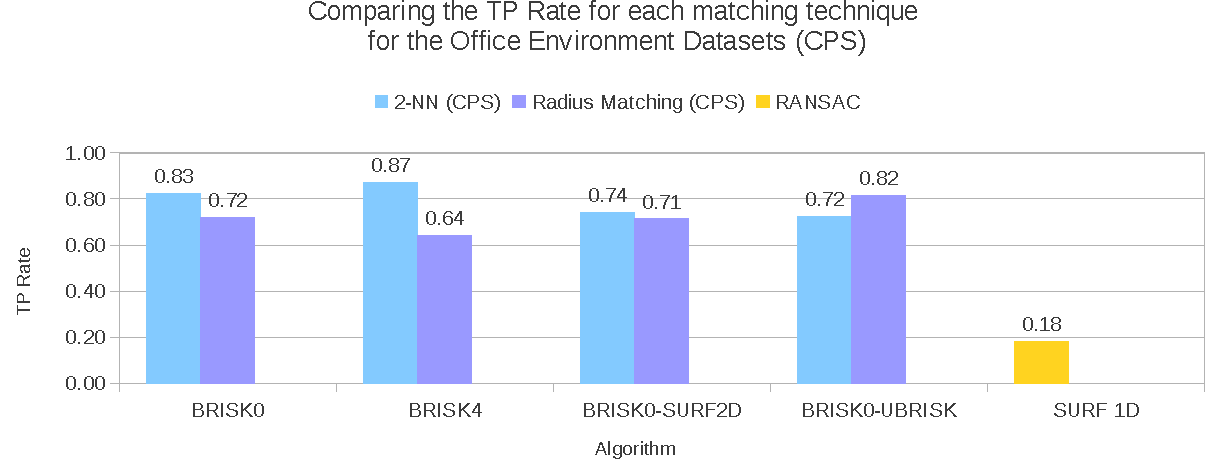
\includegraphics[width=1.0\textwidth]{../Drawings/Graphs/tp_rate_oe_cps.pdf}
    \caption{The $TP_{FP=0}^{max}$ rate for the Office Environment datasets} 
    \label{app:tp_rate_oe}
\end{figure}


\begin{table}
\caption{The number of Image Zero Matches (IZMs) for each feature extraction
algorithm using 2-NN and Radius Matching in the Office Environment}
\begin{tabular}{|c|c|}
\hline 
\textbf{Method} & \multicolumn{1}{c|}{\textbf{Image Zero Matches}}\tabularnewline
\hline 
 & \multicolumn{1}{c|}{\textbf{2-NN Matching}}\tabularnewline
\hline 
 & \textbf{CPS}\tabularnewline
\hline 
\hline 
BRISK0 & 6.00\tabularnewline
\hline 
BRISK & 5.00\tabularnewline
\hline 
BRISK0- SURF2D & 0.00\tabularnewline
\hline 
UBRISK & 27.00\tabularnewline
\hline 
1D SURF & 0.00\tabularnewline
\hline 
 & \multicolumn{1}{c|}{\textbf{Radius Matching}}\tabularnewline
\hline 
BRISK0 & 10.00\tabularnewline
\hline 
BRISK & 0.00\tabularnewline
\hline 
BRISK0- SURF2D & 7.00\tabularnewline
\hline 
UBRISK & 6.00\tabularnewline
\hline 
1D SURF & 0.00\tabularnewline
\hline 
\end{tabular}
\label{app:oe_izm}
\end{table}


\subsection{Large Hall Environment}
\label{app:lh}

\begin{figure}[ht!]
\begin{minipage}[b]{0.5\linewidth}
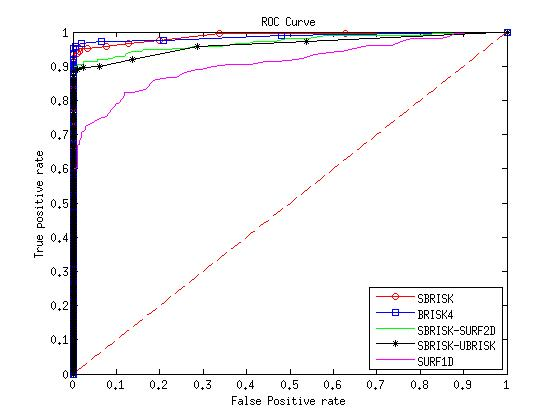
\includegraphics[scale=0.4]{../Drawings/dataset3_ROC_General_KNN_Consistent.jpg}
\caption{A comparison of the ROC curves in the large hall environment using the CPS thresholds}
\label{fig:compareKnnConsistentOffice3}
\end{minipage}
\hspace{0.5cm}
\begin{minipage}[b]{0.5\linewidth}
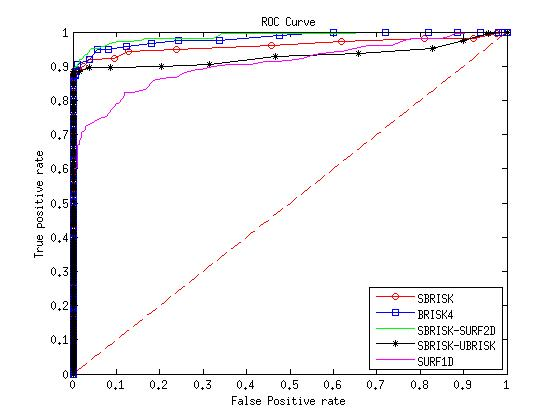
\includegraphics[scale=0.4]{../Drawings/dataset3_ROC_General_Hamming_Consistent.jpg}
\caption{A comparison of the ROC curves in the large hall environment using the CPS Hamming/Euclidean distance thresholds}
\label{fig:compareHammingConsistentOffice3}
\end{minipage}
\end{figure}

\begin{table}
\caption{The AUC and performance statistics for the Large Hall Environment
Datasets using 2-NN Matching and CPS parameters}
\begin{tabular}{|c|c|c|c|c|c|c|c|}
\hline 
\textbf{Method (2-NN)} & \textbf{Parameters} & \textbf{\% AUC} & \textbf{Detection} & \textbf{Extraction} & \textbf{Matching} & \textbf{Verification} & \textbf{Overall}\tabularnewline
 &  &  & \textbf{Time (ms)} & \textbf{Time (ms)} & \textbf{Time (ms)} & \textbf{Time (ms)} & \textbf{Time (ms)}\tabularnewline
\hline 
\hline 
BRISK0 & CPS & 98.798 & 5.412 & 22.181 & 81.944 & 0.306 & 114.365\tabularnewline
\hline 
BRISK4 & CPS & 98.703 & 28.349 & 23.880 & 83.456 & 0.298 & 140.463\tabularnewline
\hline 
BRISK0-SURF2D & CPS & 97.024 & 5.443 & 42.449 & 14.060 & 0.349 & 66.809\tabularnewline
\hline 
BRISK0-UBRISK & CPS & 96.186 & 4.787 & 7.248 & 46.827 & 0.232 & 63.541\tabularnewline
\hline 
\end{tabular}
\label{app:lh_hamming}
\end{table}


\begin{table}
\caption{The AUC and performance statistics for the Large Hall Environment
Datasets using Radius Matching and CPS parameters}
\begin{tabular}{|c|c|c|c|c|c|c|c|}
\hline 
\textbf{Method (2-NN)} & \textbf{Parameters} & \textbf{\% AUC} & \textbf{Detection} & \textbf{Extraction} & \textbf{Matching} & \textbf{Verification} & \textbf{Overall}\tabularnewline
 &  &  & \textbf{Time (ms)} & \textbf{Time (ms)} & \textbf{Time (ms)} & \textbf{Time (ms)} & \textbf{Time (ms)}\tabularnewline
\hline 
\hline 
BRISK0 & CPS & 96.070 & 3.268 & 4.762 & 2.618 & 0.028 & 15.091\tabularnewline
\hline 
BRISK4 & CPS & 98.269 & 12.123 & 6.139 & 4.359 & 0.045 & 27.164\tabularnewline
\hline 
BRISK0-SURF2D & CPS & 98.786 & 3.603 & 13.475 & 1.717 & 0.051 & 23.414\tabularnewline
\hline 
BRISK0-UBRISK & CPS & 92.964 & 3.303 & 2.581 & 2.618 & 0.030 & 13.503\tabularnewline
\hline 
\end{tabular}
\label{app:lh_hamming}
\end{table}



\begin{table}
\caption{The number of Image Zero Matches (IZMs) for each feature extraction
algorithm using 2-NN and Radius Matching in the Large Environment}


\begin{tabular}{|c|c|}
\hline 
\textbf{Method} & \multicolumn{1}{c|}{\textbf{Image Zero Matches}}\tabularnewline
\hline 
 & \multicolumn{1}{c|}{\textbf{2-NN Matching}}\tabularnewline
\hline 
 & \textbf{CPS}\tabularnewline
\hline 
\hline 
BRISK0 & 0.00\tabularnewline
\hline 
BRISK & 1.00\tabularnewline
\hline 
BRISK0- SURF2D & 0.00\tabularnewline
\hline 
UBRISK & 1.00\tabularnewline
\hline 
1D SURF & 0.00\tabularnewline
\hline 
 & \multicolumn{1}{c|}{\textbf{Radius Matching}}\tabularnewline
\hline 
BRISK0 & 0.00\tabularnewline
\hline 
BRISK & 0.00\tabularnewline
\hline 
BRISK0- SURF2D & 0.00\tabularnewline
\hline 
UBRISK & 0.00\tabularnewline
\hline 
1D SURF & 0.00\tabularnewline
\hline 
\end{tabular}
\label{app:lh_izm}
\end{table}


\begin{figure}
  \centering
    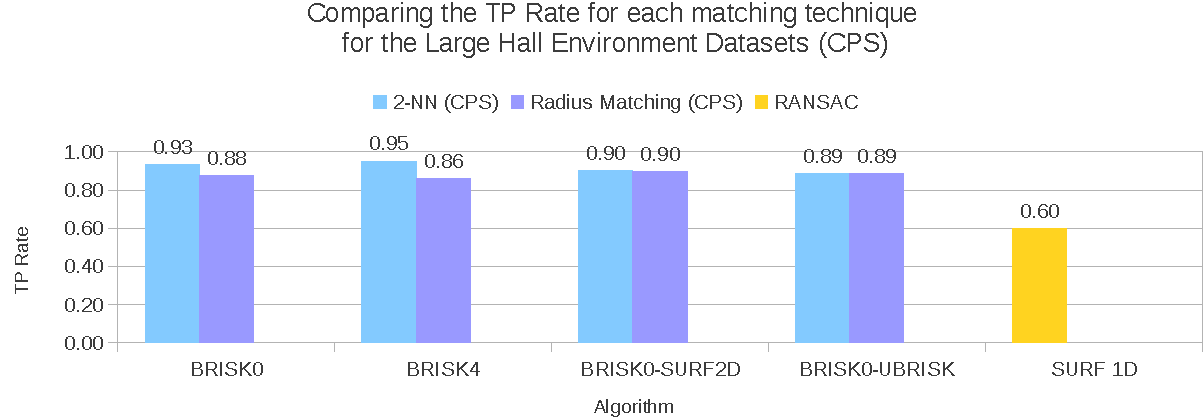
\includegraphics[width=1.0\textwidth]{../Drawings/Graphs/tp_rate_lh_cps.pdf}
    \caption{The $TP_{FP=0}^{max}$ rate for the Large Hall Environment datasets} 
    \label{app:tp_rate_lh}
\end{figure}